\documentclass[]{article}
\usepackage{lmodern}
\usepackage{amssymb,amsmath}
\usepackage{ifxetex,ifluatex}
\usepackage{fixltx2e} % provides \textsubscript
\ifnum 0\ifxetex 1\fi\ifluatex 1\fi=0 % if pdftex
  \usepackage[T1]{fontenc}
  \usepackage[utf8]{inputenc}
\else % if luatex or xelatex
  \ifxetex
    \usepackage{mathspec}
  \else
    \usepackage{fontspec}
  \fi
  \defaultfontfeatures{Ligatures=TeX,Scale=MatchLowercase}
  \newcommand{\euro}{€}
\fi
% use upquote if available, for straight quotes in verbatim environments
\IfFileExists{upquote.sty}{\usepackage{upquote}}{}
% use microtype if available
\IfFileExists{microtype.sty}{%
\usepackage{microtype}
\UseMicrotypeSet[protrusion]{basicmath} % disable protrusion for tt fonts
}{}
\usepackage[margin=1in]{geometry}
\usepackage{hyperref}
\PassOptionsToPackage{usenames,dvipsnames}{color} % color is loaded by hyperref
\hypersetup{unicode=true,
            pdftitle={Trabajo de prácticas 3},
            pdfauthor={Miguel López Campos},
            pdfborder={0 0 0},
            breaklinks=true}
\urlstyle{same}  % don't use monospace font for urls
\usepackage{color}
\usepackage{fancyvrb}
\newcommand{\VerbBar}{|}
\newcommand{\VERB}{\Verb[commandchars=\\\{\}]}
\DefineVerbatimEnvironment{Highlighting}{Verbatim}{commandchars=\\\{\}}
% Add ',fontsize=\small' for more characters per line
\usepackage{framed}
\definecolor{shadecolor}{RGB}{248,248,248}
\newenvironment{Shaded}{\begin{snugshade}}{\end{snugshade}}
\newcommand{\KeywordTok}[1]{\textcolor[rgb]{0.13,0.29,0.53}{\textbf{{#1}}}}
\newcommand{\DataTypeTok}[1]{\textcolor[rgb]{0.13,0.29,0.53}{{#1}}}
\newcommand{\DecValTok}[1]{\textcolor[rgb]{0.00,0.00,0.81}{{#1}}}
\newcommand{\BaseNTok}[1]{\textcolor[rgb]{0.00,0.00,0.81}{{#1}}}
\newcommand{\FloatTok}[1]{\textcolor[rgb]{0.00,0.00,0.81}{{#1}}}
\newcommand{\ConstantTok}[1]{\textcolor[rgb]{0.00,0.00,0.00}{{#1}}}
\newcommand{\CharTok}[1]{\textcolor[rgb]{0.31,0.60,0.02}{{#1}}}
\newcommand{\SpecialCharTok}[1]{\textcolor[rgb]{0.00,0.00,0.00}{{#1}}}
\newcommand{\StringTok}[1]{\textcolor[rgb]{0.31,0.60,0.02}{{#1}}}
\newcommand{\VerbatimStringTok}[1]{\textcolor[rgb]{0.31,0.60,0.02}{{#1}}}
\newcommand{\SpecialStringTok}[1]{\textcolor[rgb]{0.31,0.60,0.02}{{#1}}}
\newcommand{\ImportTok}[1]{{#1}}
\newcommand{\CommentTok}[1]{\textcolor[rgb]{0.56,0.35,0.01}{\textit{{#1}}}}
\newcommand{\DocumentationTok}[1]{\textcolor[rgb]{0.56,0.35,0.01}{\textbf{\textit{{#1}}}}}
\newcommand{\AnnotationTok}[1]{\textcolor[rgb]{0.56,0.35,0.01}{\textbf{\textit{{#1}}}}}
\newcommand{\CommentVarTok}[1]{\textcolor[rgb]{0.56,0.35,0.01}{\textbf{\textit{{#1}}}}}
\newcommand{\OtherTok}[1]{\textcolor[rgb]{0.56,0.35,0.01}{{#1}}}
\newcommand{\FunctionTok}[1]{\textcolor[rgb]{0.00,0.00,0.00}{{#1}}}
\newcommand{\VariableTok}[1]{\textcolor[rgb]{0.00,0.00,0.00}{{#1}}}
\newcommand{\ControlFlowTok}[1]{\textcolor[rgb]{0.13,0.29,0.53}{\textbf{{#1}}}}
\newcommand{\OperatorTok}[1]{\textcolor[rgb]{0.81,0.36,0.00}{\textbf{{#1}}}}
\newcommand{\BuiltInTok}[1]{{#1}}
\newcommand{\ExtensionTok}[1]{{#1}}
\newcommand{\PreprocessorTok}[1]{\textcolor[rgb]{0.56,0.35,0.01}{\textit{{#1}}}}
\newcommand{\AttributeTok}[1]{\textcolor[rgb]{0.77,0.63,0.00}{{#1}}}
\newcommand{\RegionMarkerTok}[1]{{#1}}
\newcommand{\InformationTok}[1]{\textcolor[rgb]{0.56,0.35,0.01}{\textbf{\textit{{#1}}}}}
\newcommand{\WarningTok}[1]{\textcolor[rgb]{0.56,0.35,0.01}{\textbf{\textit{{#1}}}}}
\newcommand{\AlertTok}[1]{\textcolor[rgb]{0.94,0.16,0.16}{{#1}}}
\newcommand{\ErrorTok}[1]{\textcolor[rgb]{0.64,0.00,0.00}{\textbf{{#1}}}}
\newcommand{\NormalTok}[1]{{#1}}
\usepackage{graphicx,grffile}
\makeatletter
\def\maxwidth{\ifdim\Gin@nat@width>\linewidth\linewidth\else\Gin@nat@width\fi}
\def\maxheight{\ifdim\Gin@nat@height>\textheight\textheight\else\Gin@nat@height\fi}
\makeatother
% Scale images if necessary, so that they will not overflow the page
% margins by default, and it is still possible to overwrite the defaults
% using explicit options in \includegraphics[width, height, ...]{}
\setkeys{Gin}{width=\maxwidth,height=\maxheight,keepaspectratio}
\setlength{\parindent}{0pt}
\setlength{\parskip}{6pt plus 2pt minus 1pt}
\setlength{\emergencystretch}{3em}  % prevent overfull lines
\providecommand{\tightlist}{%
  \setlength{\itemsep}{0pt}\setlength{\parskip}{0pt}}
\setcounter{secnumdepth}{0}

%%% Use protect on footnotes to avoid problems with footnotes in titles
\let\rmarkdownfootnote\footnote%
\def\footnote{\protect\rmarkdownfootnote}

%%% Change title format to be more compact
\usepackage{titling}

% Create subtitle command for use in maketitle
\newcommand{\subtitle}[1]{
  \posttitle{
    \begin{center}\large#1\end{center}
    }
}

\setlength{\droptitle}{-2em}
  \title{Trabajo de prácticas 3}
  \pretitle{\vspace{\droptitle}\centering\huge}
  \posttitle{\par}
  \author{Miguel López Campos}
  \preauthor{\centering\large\emph}
  \postauthor{\par}
  \predate{\centering\large\emph}
  \postdate{\par}
  \date{4 de mayo de 2016}



% Redefines (sub)paragraphs to behave more like sections
\ifx\paragraph\undefined\else
\let\oldparagraph\paragraph
\renewcommand{\paragraph}[1]{\oldparagraph{#1}\mbox{}}
\fi
\ifx\subparagraph\undefined\else
\let\oldsubparagraph\subparagraph
\renewcommand{\subparagraph}[1]{\oldsubparagraph{#1}\mbox{}}
\fi

\begin{document}
\maketitle

\section{Ejercicio 1}\label{ejercicio-1}

\subsection{Apartados a y b}\label{apartados-a-y-b}

Para trabajar con la base de datos Auto solo tenemos que importar la
librería ISLR y llamar al comando Auto que directamente nos devuelve el
data frame correspondiente a la base de datos. Yo lo introduciré en una
variable llamada `auto'.

\begin{Shaded}
\begin{Highlighting}[]
\NormalTok{##Ejercicio 1}
\NormalTok{##Apartados a y b}
\NormalTok{auto <-}\StringTok{ }\NormalTok{Auto}
\KeywordTok{pairs}\NormalTok{(auto, }\DataTypeTok{col=}\StringTok{"blue"}\NormalTok{)}
\end{Highlighting}
\end{Shaded}

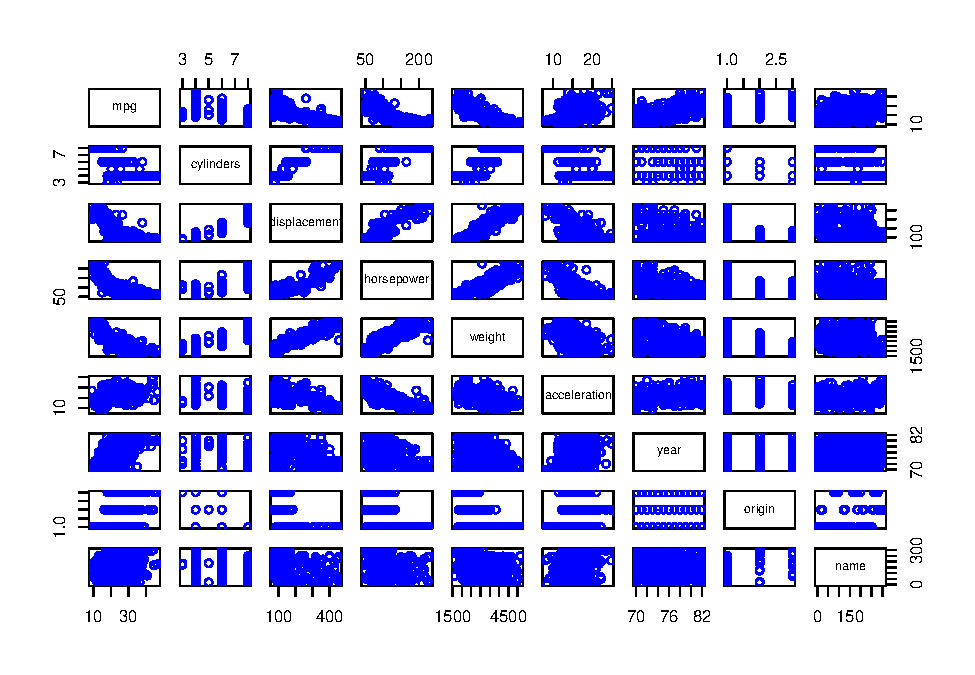
\includegraphics{TrabajoPracticas3_files/figure-latex/unnamed-chunk-2-1.pdf}

Como podemos ver, la característica mpg parece tener cierta relación
lineal con el `displacement' (cilindrada), `horsepower'(potencia en
caballos de vapor) y `weight' (peso), ya que en las tres gráficas parece
apreciarse que cuando el valor de una característica aumenta el de la
otra disminuye. En las siguientes gráficas se puede observar mejor.

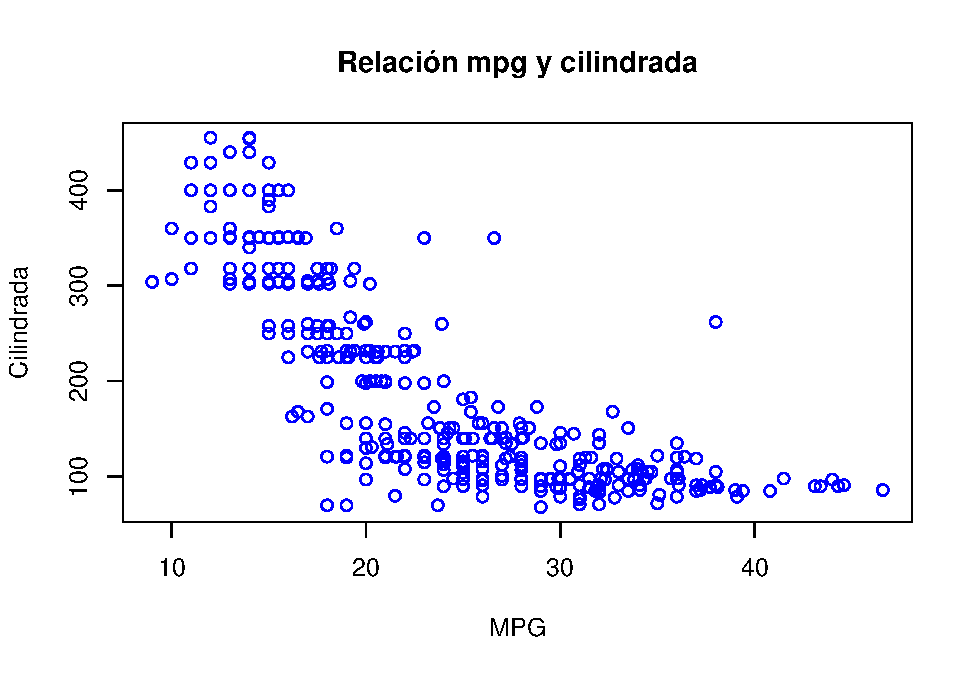
\includegraphics{TrabajoPracticas3_files/figure-latex/unnamed-chunk-4-1.pdf}

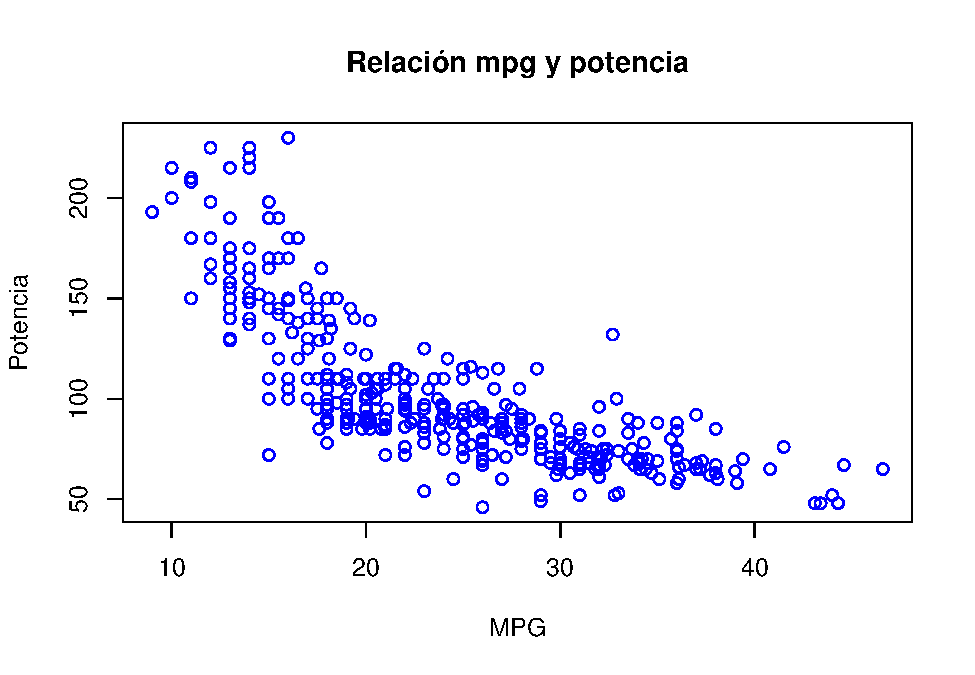
\includegraphics{TrabajoPracticas3_files/figure-latex/unnamed-chunk-6-1.pdf}

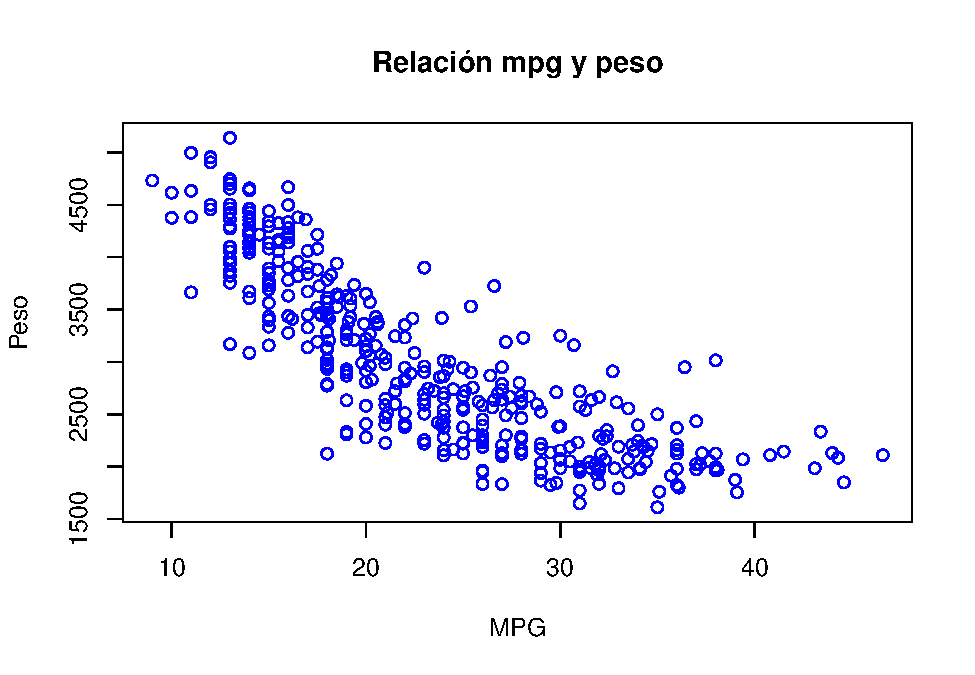
\includegraphics{TrabajoPracticas3_files/figure-latex/unnamed-chunk-8-1.pdf}

Pensándolo de otra manera, dejando aparte las gráficas, tiene sentido
decir que el consumo depende de estos tres factores, a si que podemos
``aceptar'' estas relaciones.

\subsection{Apartados c y d}\label{apartados-c-y-d}

Hago un nuevo data frame con las características elegidas y
posteriormente realizo el etiquetado según el enunciado: para Knn, si el
MPG está por encima de la mediana le asigno etiqueta +1 y si está por
debajo, etiqueta -1. Para regresión logística etiquetaré con 0 y 1 como
a continuación hago. Para extraer una submuestra empleo la función
sample, cogiendo el 80\% de índices del conjunto de datos. Los restantes
serán el test set.

\begin{Shaded}
\begin{Highlighting}[]
\NormalTok{###Apartados c y d}
\NormalTok{##Hago el etiquetado (0,1 para LR y -1 y +1 para knn)}
\KeywordTok{set.seed}\NormalTok{(}\DecValTok{1}\NormalTok{)}
\NormalTok{mediana <-}\StringTok{ }\KeywordTok{median}\NormalTok{(auto$mpg)}
\NormalTok{datos <-}\StringTok{ }\KeywordTok{data.frame}\NormalTok{(auto$displacement, auto$weight, auto$horsepower)}
\NormalTok{training_ind <-}\StringTok{ }\KeywordTok{sample}\NormalTok{(}\DataTypeTok{x=}\NormalTok{(}\DecValTok{1}\NormalTok{:}\KeywordTok{nrow}\NormalTok{(datos)), }\DataTypeTok{size=}\FloatTok{0.8}\NormalTok{*}\KeywordTok{nrow}\NormalTok{(datos))}
\NormalTok{training <-}\StringTok{ }\NormalTok{datos[training_ind,]}
\NormalTok{test <-}\StringTok{ }\NormalTok{datos[-training_ind,]}
\NormalTok{label_training <-}\StringTok{ }\NormalTok{auto$mpg[training_ind]}
\NormalTok{label_test <-}\StringTok{ }\NormalTok{auto$mpg[-training_ind]}
\NormalTok{positivos <-}\StringTok{ }\NormalTok{label_training>mediana}
\NormalTok{label_training[positivos] <-}\StringTok{ }\DecValTok{1}
\NormalTok{label_training[!positivos] <-}\StringTok{ }\DecValTok{0}
\NormalTok{positivos <-}\StringTok{ }\NormalTok{label_test>mediana}
\NormalTok{label_test[positivos] <-}\StringTok{ }\DecValTok{1}
\NormalTok{label_test[!positivos] <-}\StringTok{ }\DecValTok{0}
\end{Highlighting}
\end{Shaded}

A continuación aplico regresión logística. Para aplicarla uso la función
glm. Esta función lo que hace es ajustar modelos lineales generalizados.
Para indicarle a R que vamos a aplicar regresión logística lo que
hacemos es introducirle el argumento `family=binomial'.

Lo que hago después es usar la función predict para hacer la
`predicción' del conjunto de datos de test. A predict le meto como
argumento el modelo ajustado con la regresión logística, el data set de
test y el parámetro type tenemos que ajustarlo a ``response'' para que
nos devuelva probabilidades. Probs, por lo tanto, será la probabilidad
de cada uno de los datos de test. Si la probabilidad es mayor que 0.5,
consideraremos que su etiqueta es 1, es decir, consumo bajo. Si es menor
que 0.5, entonces consideraremos que será consumo alto.

\begin{Shaded}
\begin{Highlighting}[]
\NormalTok{##Aplico glm (regresión logística)}
\KeywordTok{set.seed}\NormalTok{(}\DecValTok{1}\NormalTok{)}

\NormalTok{model <-}\StringTok{ }\KeywordTok{glm}\NormalTok{(}\DataTypeTok{formula=}\NormalTok{label_training~.,}\DataTypeTok{family=}\NormalTok{binomial,}\DataTypeTok{data=}\NormalTok{training)}
\KeywordTok{summary}\NormalTok{(model)}
\end{Highlighting}
\end{Shaded}

\begin{verbatim}
## 
## Call:
## glm(formula = label_training ~ ., family = binomial, data = training)
## 
## Deviance Residuals: 
##     Min       1Q   Median       3Q      Max  
## -2.3586  -0.3148  -0.0034   0.3702   3.3607  
## 
## Coefficients:
##                     Estimate Std. Error z value Pr(>|z|)    
## (Intercept)       11.7934871  1.8081615   6.522 6.92e-11 ***
## auto.displacement -0.0124994  0.0057158  -2.187  0.02876 *  
## auto.weight       -0.0017599  0.0007688  -2.289  0.02206 *  
## auto.horsepower   -0.0495878  0.0151868  -3.265  0.00109 ** 
## ---
## Signif. codes:  0 '***' 0.001 '**' 0.01 '*' 0.05 '.' 0.1 ' ' 1
## 
## (Dispersion parameter for binomial family taken to be 1)
## 
##     Null deviance: 433.65  on 312  degrees of freedom
## Residual deviance: 173.54  on 309  degrees of freedom
## AIC: 181.54
## 
## Number of Fisher Scoring iterations: 7
\end{verbatim}

\begin{Shaded}
\begin{Highlighting}[]
\NormalTok{##Con predict calculo las probabilidades}
\NormalTok{probs <-}\StringTok{ }\KeywordTok{predict}\NormalTok{(model,test,}\DataTypeTok{type=}\StringTok{"response"}\NormalTok{)}
\NormalTok{##Hago el error de clasificación}
\NormalTok{label_prediction <-}\StringTok{ }\NormalTok{probs}
\NormalTok{label_prediction[label_prediction>=}\FloatTok{0.5}\NormalTok{] <-}\StringTok{ }\DecValTok{1}
\NormalTok{label_prediction[label_prediction<}\FloatTok{0.5}\NormalTok{] <-}\StringTok{ }\DecValTok{0}
\NormalTok{error <-}\StringTok{ }\NormalTok{label_test!=label_prediction}
\NormalTok{error <-}\StringTok{ }\NormalTok{error[error==}\OtherTok{TRUE}\NormalTok{]}
\NormalTok{error <-}\StringTok{ }\KeywordTok{length}\NormalTok{(error)/}\KeywordTok{length}\NormalTok{(label_test)}
\NormalTok{error}
\end{Highlighting}
\end{Shaded}

\begin{verbatim}
## [1] 0.08860759
\end{verbatim}

Como vemos el error que es de un 8\%.

Ahora aplicaremos k-nn. Este algoritmo es un algoritmo de aprendizaje
por semejanza. Lo que hace es calcular la distancia euclídea entre los
datos de training y el que queremos predecir, y los k vecinos más
cercanos dirán por voto mayoritario a qué clase pertenece el vector de
características que queremos predecir. Para aplicar k-nn usaremos la
función knn de la librería `class'. Antes de emplearlo tenemos que
normalizar los datos. Para normalizar los datos emplearé la fución
normalizar, implementada por mí:

\begin{Shaded}
\begin{Highlighting}[]
\CommentTok{#Función que normaliza un conjunto de datos}
\NormalTok{normalizar <-}\StringTok{ }\NormalTok{function(datos)}
\NormalTok{\{}
  \NormalTok{for(i in }\DecValTok{1}\NormalTok{:}\KeywordTok{ncol}\NormalTok{(datos))}
  \NormalTok{\{}
    \NormalTok{minimo <-}\StringTok{ }\KeywordTok{min}\NormalTok{(datos[,i], }\DataTypeTok{na.rm=}\OtherTok{TRUE}\NormalTok{)}
    \NormalTok{maximo <-}\StringTok{ }\KeywordTok{max}\NormalTok{(datos[,i], }\DataTypeTok{na.rm=}\OtherTok{TRUE}\NormalTok{)}
    
    \NormalTok{if(minimo ==}\StringTok{ }\DecValTok{0} \NormalTok{&&}\StringTok{ }\NormalTok{maximo==}\DecValTok{0}\NormalTok{)\{datos[,i]<-}\DecValTok{0}\NormalTok{\}else}
    \NormalTok{\{}
      \NormalTok{datos[,i] <-}\StringTok{ }\NormalTok{(datos[,i]-minimo)/(maximo-minimo)}
    \NormalTok{\}}
  \NormalTok{\}}
  
  \KeywordTok{return}\NormalTok{(datos)}
\NormalTok{\}}
\end{Highlighting}
\end{Shaded}

A continuación normalizo los datos. Después particiono los datos,
dejando los mismos conjuntos de training y test que cuando he aplicado
regresión logística. Para ello uso los mismos índices que he usado
anteriormente.

Para aplicar knn usamos la función knn de la librería ``class''. A esta
función le introducimos el training dataset y el test dataset como
argumentos, además del valor de k y el vector de etiquetas de training.
La función nos devolverá un vector que será la clasificación que el
algoritmo ha predicho.

En este caso, como ya no estamos prediciendo probabilidades, las
etiquetas serán -1 (en el caso de que el consumo sea alto) y +1 (en el
caso de que el consumo sea bajo).

\begin{Shaded}
\begin{Highlighting}[]
\NormalTok{##A continuación aplicamos knn}
\KeywordTok{set.seed}\NormalTok{(}\DecValTok{1}\NormalTok{)}

\NormalTok{datos_normalizados <-}\StringTok{ }\KeywordTok{normalizar}\NormalTok{(datos)}
\NormalTok{##}
\NormalTok{##}
\NormalTok{training_knn <-}\StringTok{ }\NormalTok{datos_normalizados[training_ind,]}
\NormalTok{test_knn <-}\StringTok{ }\NormalTok{datos_normalizados[-training_ind,]}
\NormalTok{label_training_knn <-}\StringTok{ }\NormalTok{label_training}
\NormalTok{label_training_knn[label_training_knn==}\DecValTok{0}\NormalTok{] <-}\StringTok{ }\NormalTok{-}\DecValTok{1}
\NormalTok{prediction <-}\StringTok{ }\KeywordTok{knn}\NormalTok{(training_knn, test_knn, }\DataTypeTok{cl=}\NormalTok{label_training_knn, }\DataTypeTok{k=}\DecValTok{3}\NormalTok{)}
\NormalTok{##########Etiquetas reales del conjunto de test}
\NormalTok{label_test_knn <-}\StringTok{ }\NormalTok{label_test}
\NormalTok{label_test_knn[label_test_knn==}\DecValTok{0}\NormalTok{] <-}\StringTok{ }\NormalTok{-}\DecValTok{1}
\NormalTok{##########Calculo el error}
\NormalTok{error <-}\StringTok{ }\NormalTok{label_test_knn[label_test_knn!=prediction]}
\NormalTok{error <-}\StringTok{ }\KeywordTok{length}\NormalTok{(error)/}\KeywordTok{length}\NormalTok{(label_test_knn)}
\NormalTok{##############################}
\NormalTok{error}
\end{Highlighting}
\end{Shaded}

\begin{verbatim}
## [1] 0.1139241
\end{verbatim}

En este caso tenemos un error de un 11\%.

Para ver cual es el valor de k que mejor ajusta los datos del knn,
usaremos la función tune.knn de la biblioteca e1071 . Para usarla
primero la variable dependiente tenemos que cambiarla por tipos de datos
lógicos, para que funcione la función. Después aplico la función
indicándole que queremos una cross validation (validación cruzada) y que
la haga 10 veces. El parámetro k variará entre 1 y 20.

\begin{Shaded}
\begin{Highlighting}[]
\NormalTok{##Aplicamos tune.knn para ver que k sería el óptimo para nuestro caso}
\NormalTok{##las etiquetas deben ser booleanos}
\NormalTok{label_training_knn[label_training_knn==-}\DecValTok{1}\NormalTok{] <-}\StringTok{ }\DecValTok{0}
\NormalTok{label_training_knn[label_training_knn==}\DecValTok{1}\NormalTok{] <-}\StringTok{ }\DecValTok{1}

\NormalTok{knn.cross <-}\StringTok{ }\KeywordTok{tune.knn}\NormalTok{(}\DataTypeTok{x =} \NormalTok{training_knn, }\DataTypeTok{y =} \KeywordTok{as.logical}\NormalTok{(label_training_knn), }\DataTypeTok{k =} \DecValTok{1}\NormalTok{:}\DecValTok{20}\NormalTok{,}
                      \DataTypeTok{tunecontrol=}\KeywordTok{tune.control}\NormalTok{(}\DataTypeTok{sampling =} \StringTok{"cross"}\NormalTok{), }\DataTypeTok{cross=}\DecValTok{10}\NormalTok{)}
\end{Highlighting}
\end{Shaded}

Resumen de tune.knn:

\begin{Shaded}
\begin{Highlighting}[]
\KeywordTok{summary}\NormalTok{(knn.cross)}
\end{Highlighting}
\end{Shaded}

\begin{verbatim}
## 
## Parameter tuning of 'knn.wrapper':
## 
## - sampling method: 10-fold cross validation 
## 
## - best parameters:
##  k
##  5
## 
## - best performance: 0.09919355 
## 
## - Detailed performance results:
##     k      error dispersion
## 1   1 0.12752016 0.09311525
## 2   2 0.13750000 0.06659536
## 3   3 0.11844758 0.07782834
## 4   4 0.10241935 0.09727483
## 5   5 0.09919355 0.08265610
## 6   6 0.10564516 0.09274169
## 7   7 0.10241935 0.08317900
## 8   8 0.11532258 0.07816268
## 9   9 0.11219758 0.08116718
## 10 10 0.11219758 0.07211565
## 11 11 0.10897177 0.07358863
## 12 12 0.11219758 0.07525389
## 13 13 0.11219758 0.07525389
## 14 14 0.11219758 0.07525389
## 15 15 0.11219758 0.08667798
## 16 16 0.11209677 0.08390559
## 17 17 0.12157258 0.08577070
## 18 18 0.12157258 0.08577070
## 19 19 0.11844758 0.08493205
## 20 20 0.11844758 0.08493205
\end{verbatim}

Ahora dibujaremos las curvas ROCR

Para k-nn:

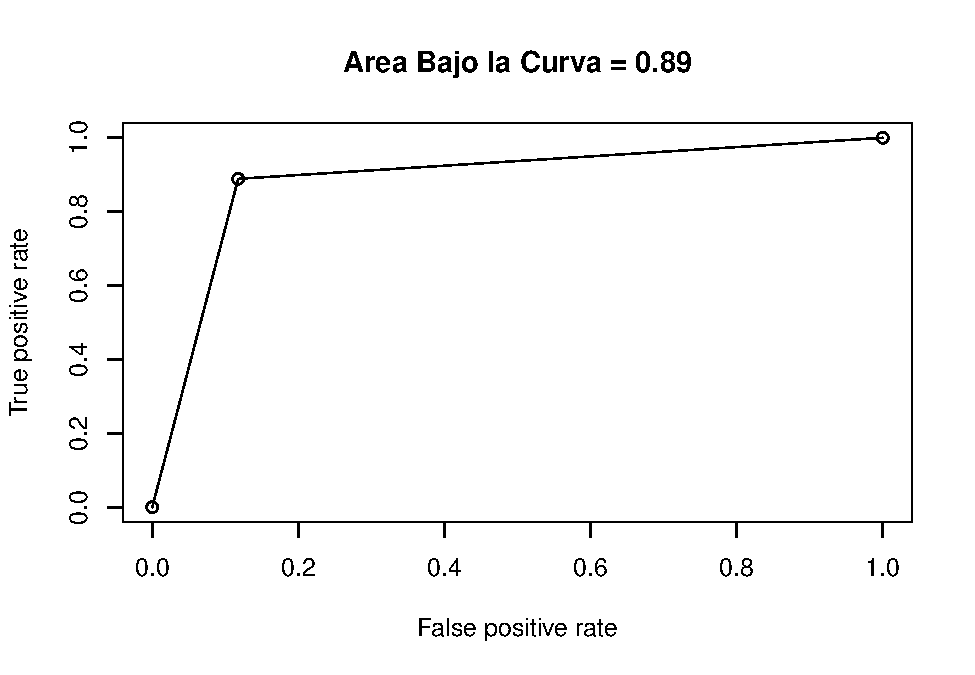
\includegraphics{TrabajoPracticas3_files/figure-latex/unnamed-chunk-19-1.pdf}

Para regresión logística:

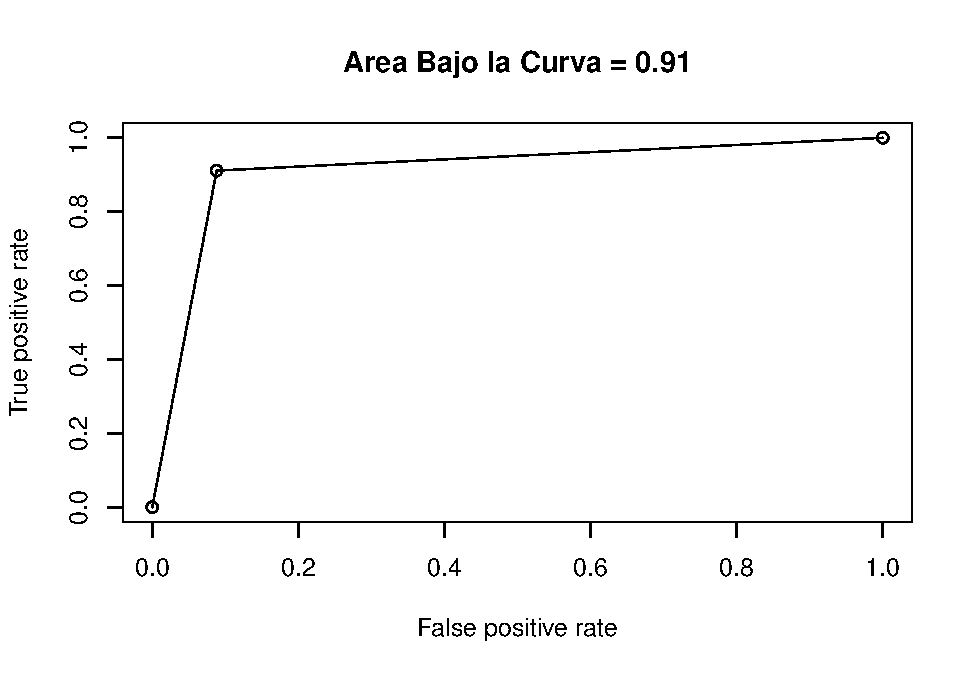
\includegraphics{TrabajoPracticas3_files/figure-latex/unnamed-chunk-21-1.pdf}

El principal dato estadístico de las curvas es el área bajo la
circunferencia (AUC). Este área representa la probabilidad de que un
clasificador puntuará una instancia positiva elegida aleatoriamente más
alta que una negativa. Por lo tanto, como podemos ver, en el modelo de
regresión logística este área es más grande y por lo tanto la
probabilidad es mayor.

\subsection{Apartado e (Bonus)}\label{apartado-e-bonus}

En este apartado calcularemos por validación cruzada el error. Cogeremos
5 particiones, por lo que en cada partición se cogerá como training el
80\% de los datos y como test el 20\% restante.

Primero haremos la regresión logística.

\begin{Shaded}
\begin{Highlighting}[]
\NormalTok{##Apartado e (Bonus)}

\CommentTok{#Primero hacemos validación cruzada para regresión logística}
\KeywordTok{set.seed}\NormalTok{(}\DecValTok{1}\NormalTok{)}

\NormalTok{probs <-}\StringTok{ }\KeywordTok{rep}\NormalTok{(}\DecValTok{1}\NormalTok{,}\KeywordTok{nrow}\NormalTok{(Auto))}
\NormalTok{errores <-}\StringTok{ }\KeywordTok{vector}\NormalTok{()}

\NormalTok{for(i in }\DecValTok{1}\NormalTok{:}\DecValTok{5}\NormalTok{)}
\NormalTok{\{}
    \NormalTok{##Saco la submuestra de test (20%)}
    \NormalTok{test <-}\StringTok{ }\KeywordTok{sample}\NormalTok{(}\DataTypeTok{x=}\DecValTok{1}\NormalTok{:}\KeywordTok{nrow}\NormalTok{(datos), }\DataTypeTok{size=}\NormalTok{(}\FloatTok{0.2}\NormalTok{*}\KeywordTok{nrow}\NormalTok{(datos)), }\DataTypeTok{prob=}\NormalTok{probs)}
    
    \NormalTok{##Pongo probs a 0 del subconjunto cogido para que no se vuelva a repetir}
    \NormalTok{probs[test] <-}\StringTok{ }\DecValTok{0}
    
    \NormalTok{mediana <-}\StringTok{ }\KeywordTok{median}\NormalTok{(Auto$mpg)}
    \NormalTok{label <-}\StringTok{ }\NormalTok{Auto$mpg}
    \NormalTok{positivos <-}\StringTok{ }\NormalTok{label>=mediana}
    \NormalTok{label[positivos] <-}\StringTok{ }\DecValTok{1}
    \NormalTok{label[!positivos] <-}\StringTok{ }\DecValTok{0}
    
    \NormalTok{label_test <-}\StringTok{ }\NormalTok{label[test]}
    \NormalTok{label_training <-}\StringTok{ }\NormalTok{label[-test]}
    
    
    \NormalTok{training_set <-}\StringTok{ }\NormalTok{datos[-test,]}
    \NormalTok{test_set <-}\StringTok{ }\NormalTok{datos[test,]}

    \NormalTok{##Aplicamos ahora la función glm sobre el training data set}
    \NormalTok{model <-}\StringTok{ }\KeywordTok{glm}\NormalTok{(}\DataTypeTok{formula=}\NormalTok{label_training ~}\StringTok{ }\NormalTok{., }\DataTypeTok{family=}\NormalTok{binomial, }\DataTypeTok{data=}\NormalTok{training_set)}
    \NormalTok{model_probs <-}\StringTok{ }\KeywordTok{predict}\NormalTok{(model,test_set,}\DataTypeTok{type=}\StringTok{"response"}\NormalTok{)}
    \NormalTok{label_prediction <-}\StringTok{ }\NormalTok{model_probs}
    \NormalTok{label_prediction[label_prediction>=}\FloatTok{0.5}\NormalTok{] <-}\StringTok{ }\DecValTok{1}
    \NormalTok{label_prediction[label_prediction<}\FloatTok{0.5}\NormalTok{] <-}\StringTok{ }\DecValTok{0}
    \NormalTok{error <-}\StringTok{ }\NormalTok{label_prediction!=label_test}
    \NormalTok{error <-}\StringTok{ }\NormalTok{error[error==}\OtherTok{TRUE}\NormalTok{]}
    \NormalTok{errores[i] <-}\StringTok{ }\KeywordTok{length}\NormalTok{(error)/}\KeywordTok{length}\NormalTok{(label_test)}
    
\NormalTok{\}}

\NormalTok{##El error promedio es el siguiente:}

\KeywordTok{mean}\NormalTok{(errores)}
\end{Highlighting}
\end{Shaded}

\begin{verbatim}
## [1] 0.1153846
\end{verbatim}

A continuación sigo el mismo procedimiento pero con el knn (con k=5, que
es el mejor k para nuestro modelo, anteriormente calculado con tune.knn)

\begin{Shaded}
\begin{Highlighting}[]
\NormalTok{##Aplicamos validación cruzada al modelo k-nn}
\KeywordTok{set.seed}\NormalTok{(}\DecValTok{1}\NormalTok{)}

\NormalTok{probs <-}\StringTok{ }\KeywordTok{rep}\NormalTok{(}\DecValTok{1}\NormalTok{,}\KeywordTok{nrow}\NormalTok{(Auto))}
\NormalTok{errores <-}\StringTok{ }\KeywordTok{vector}\NormalTok{()}

\NormalTok{for(i in }\DecValTok{1}\NormalTok{:}\DecValTok{5}\NormalTok{)}
\NormalTok{\{}
   \NormalTok{##Saco la submuestra de test (20%)}
    \NormalTok{test <-}\StringTok{ }\KeywordTok{sample}\NormalTok{(}\DataTypeTok{x=}\DecValTok{1}\NormalTok{:}\KeywordTok{nrow}\NormalTok{(datos), }\DataTypeTok{size=}\NormalTok{(}\FloatTok{0.2}\NormalTok{*}\KeywordTok{nrow}\NormalTok{(datos)), }\DataTypeTok{prob=}\NormalTok{probs)}
    
    \NormalTok{##Pongo probs a 0 del subconjunto cogido para que no se vuelva a repetir}
    \NormalTok{probs[test] <-}\StringTok{ }\DecValTok{0}
    
    \NormalTok{##Realizo el etiquetado}
    \NormalTok{mediana <-}\StringTok{ }\KeywordTok{median}\NormalTok{(Auto$mpg)}
    \NormalTok{label <-}\StringTok{ }\NormalTok{Auto$mpg}
    \NormalTok{positivos <-}\StringTok{ }\NormalTok{label>=mediana}
    \NormalTok{label[positivos] <-}\StringTok{ }\DecValTok{1}
    \NormalTok{label[!positivos] <-}\StringTok{ }\NormalTok{-}\DecValTok{1}
    
    \NormalTok{label_test <-}\StringTok{ }\NormalTok{label[test]}
    \NormalTok{label_training <-}\StringTok{ }\NormalTok{label[-test]}
    
    \NormalTok{training_set <-}\StringTok{ }\NormalTok{datos_normalizados[-test,]}
    \NormalTok{test_set <-}\StringTok{ }\NormalTok{datos_normalizados[test,]}
    \NormalTok{##Aplicamos la funcion k-nn}
    \NormalTok{prediction <-}\StringTok{ }\KeywordTok{knn}\NormalTok{(training_set, test_set, }\DataTypeTok{cl=}\NormalTok{label_training, }\DataTypeTok{k=}\DecValTok{5}\NormalTok{)}
    
    \NormalTok{##Vemos el error}
    \NormalTok{error <-}\StringTok{ }\NormalTok{prediction[prediction!=label_test]}
    \NormalTok{errores[i] <-}\StringTok{ }\KeywordTok{length}\NormalTok{(error)/}\KeywordTok{length}\NormalTok{(label_test)}
\NormalTok{\}}

\KeywordTok{mean}\NormalTok{(errores)}
\end{Highlighting}
\end{Shaded}

\begin{verbatim}
## [1] 0.09230769
\end{verbatim}

\section{Ejercicio 2}\label{ejercicio-2}

Para trabajar con la base de datos Boston, tengo que cargar el paquete
`MASS'. Guardaré la base de datos en una variable llamada dataBoston.
Para realizar este ejercicio he tomado como fuente el libro ISLR que hay
en decsai.

\begin{Shaded}
\begin{Highlighting}[]
\NormalTok{############EJERCICIO 2}
\NormalTok{dataBoston <-}\StringTok{ }\NormalTok{Boston}
\end{Highlighting}
\end{Shaded}

\subsection{Apartado a}\label{apartado-a}

A continuación, para hacer una selección de características, emplearé un
modelo de regresión Lasso. Para ello usaré el paquete `glmnet'. Mediante
validación cruzada averiguamos el mejor lambda, ya que glmnet aplica el
modelo para varios lambdas, dados como argumento o por defecto. Mediante
predict hacemos una `predicción' de los coeficientes y le daremos como
argumento el mejor lambda calculado por cross validation. Para ver
cuales son relevantes, cogeremos aquellos cuyo valor absoluto sea mayor
al umbral \(10^{-2}\). Usaremos crim como variable continua.

\begin{Shaded}
\begin{Highlighting}[]
\NormalTok{##Apartado a}
\KeywordTok{set.seed}\NormalTok{(}\DecValTok{1}\NormalTok{)}
\NormalTok{##Creo un array que será nuestro Y (variable que predeciremos)}

\NormalTok{label_boston <-}\StringTok{ }\NormalTok{dataBoston$crim}
\NormalTok{##Elimino del dataset la columna que consideraremos etiqueta}

\NormalTok{dataBoston <-}\StringTok{ }\NormalTok{dataBoston[,-}\DecValTok{1}\NormalTok{]}


\NormalTok{##Aplico el modelo lasso sobre todo el conjunto de datos.}
\NormalTok{##Para aplicar regresión Lasso, tenemos que elegir el parámetro}
\NormalTok{##alpha de la función glmnet como '1'. Primero averiguo mediante}
\NormalTok{##Validación cuzada el mejor lambda posible}

\NormalTok{modelo_lasso <-}\StringTok{ }\KeywordTok{cv.glmnet}\NormalTok{(}\KeywordTok{as.matrix}\NormalTok{(dataBoston), label_boston, }\DataTypeTok{alpha=}\DecValTok{1}\NormalTok{)}
\NormalTok{mejor_lambda <-}\StringTok{ }\NormalTok{modelo_lasso$lambda.min}


\NormalTok{##A continuación aplico regresión lasso y hago una predicción de los}
\NormalTok{##coeficientes para el mejor lambda anteriormente calculado}
\NormalTok{##A glmnet hay que pasar el dataSet como una matriz}

\NormalTok{out <-}\StringTok{ }\KeywordTok{glmnet}\NormalTok{(}\KeywordTok{as.matrix}\NormalTok{(dataBoston), label_boston, }\DataTypeTok{alpha=}\DecValTok{1}\NormalTok{)}
\NormalTok{coefs <-}\StringTok{ }\KeywordTok{predict}\NormalTok{(out, }\DataTypeTok{type=}\StringTok{"coefficients"}\NormalTok{, }\DataTypeTok{s=}\NormalTok{mejor_lambda)}


\NormalTok{##Valor de los coeficientes:}
\NormalTok{coefs}
\end{Highlighting}
\end{Shaded}

\begin{verbatim}
## 14 x 1 sparse Matrix of class "dgCMatrix"
##                        1
## (Intercept) 14.428038932
## zn           0.039364727
## indus       -0.071259165
## chas        -0.641610611
## nox         -8.404034511
## rm           0.321491735
## age          .          
## dis         -0.875434881
## rad          0.538512550
## tax         -0.001104582
## ptratio     -0.223867381
## black       -0.007540242
## lstat        0.127002383
## medv        -0.174760563
\end{verbatim}

\begin{Shaded}
\begin{Highlighting}[]
\NormalTok{##Cogeremos los coeficientes cuyo valor absoluto sea mayor que}
\NormalTok{##el umbral 10^-2}
\NormalTok{coeficientes_validos <-}\StringTok{ }\NormalTok{coefs[}\DecValTok{2}\NormalTok{:}\KeywordTok{nrow}\NormalTok{(coefs),]}
\NormalTok{coeficientes_validos <-}\StringTok{ }\KeywordTok{abs}\NormalTok{(coeficientes_validos)>=}\DecValTok{10}\NormalTok{^-}\DecValTok{2}
\end{Highlighting}
\end{Shaded}

Ya tenemos los coeficientes que son más grandes que el umbral propuesto.
Ahora tenemos que eliminar las características que no lo superan:

\begin{Shaded}
\begin{Highlighting}[]
\NormalTok{dataBoston <-}\StringTok{ }\NormalTok{dataBoston[,coeficientes_validos]}

\NormalTok{##Nos quedamos con 10 características}
\end{Highlighting}
\end{Shaded}

Finalmente nos quedamos con 10 características (de las 13 que había
inicialmente).

\subsection{Apartado b}\label{apartado-b}

Ahora ajustaremos un modelo de regresión regularizada con
``weight-decay'' (ridge-regression). Usaremos las variables
seleccionadas por el modelo Lasso. Para aplicar este modelo de regresión
regularizada, emplearemos la misma función que para el modelo Lasso
(glmnet), pero como parámetro elegiremos alpha=0 (que indica que
queremos realizar una regresión ridge).

Primero, al igual que al aplicar Lasso, buscaremos el mejor lambda
posible mediante Cross-validation.

\begin{Shaded}
\begin{Highlighting}[]
\NormalTok{##Apartado b}

\KeywordTok{set.seed}\NormalTok{(}\DecValTok{1}\NormalTok{)}
\NormalTok{##Averiguo mejor lambda}

\NormalTok{ridge.cv <-}\StringTok{ }\KeywordTok{cv.glmnet}\NormalTok{(}\KeywordTok{as.matrix}\NormalTok{(dataBoston), label_boston, }\DataTypeTok{alpha=}\DecValTok{0}\NormalTok{)}
\NormalTok{mejor_lambda <-}\StringTok{ }\NormalTok{ridge.cv$lambda.min}

\NormalTok{##Aplicamos ahora regresión ridge}
\NormalTok{##Predecimos los coeficientes de la misma manera que en el modelo lasso}
\NormalTok{##con la función predict}

\NormalTok{out <-}\StringTok{ }\KeywordTok{glmnet}\NormalTok{(}\KeywordTok{as.matrix}\NormalTok{(dataBoston), label_boston, }\DataTypeTok{alpha=}\DecValTok{0}\NormalTok{)}
\NormalTok{coefs <-}\StringTok{ }\KeywordTok{predict}\NormalTok{(out, }\DataTypeTok{type=}\StringTok{"coefficients"}\NormalTok{, }\DataTypeTok{s=}\NormalTok{mejor_lambda)}
\NormalTok{coefs <-}\StringTok{ }\NormalTok{coefs[}\DecValTok{1}\NormalTok{:}\KeywordTok{nrow}\NormalTok{(coefs),]}

\NormalTok{##Los coeficientes (pesos) son los siguientes}
\NormalTok{coefs}
\end{Highlighting}
\end{Shaded}

\begin{verbatim}
## (Intercept)          zn       indus        chas         nox          rm 
##  5.20805729  0.03632933 -0.05140127 -0.91377317 -4.09499387  0.50968577 
##         dis         rad     ptratio       lstat        medv 
## -0.71150058  0.48490279 -0.14050335  0.15576203 -0.16028160
\end{verbatim}

\begin{Shaded}
\begin{Highlighting}[]
\NormalTok{##A continución calculamos la predicción con predict}
\NormalTok{##y posteriormente el error residual cuadrático}
\NormalTok{prediccion <-}\StringTok{ }\KeywordTok{predict}\NormalTok{(out, }\DataTypeTok{s=}\NormalTok{mejor_lambda, }\DataTypeTok{newx=}\KeywordTok{as.matrix}\NormalTok{(dataBoston))}

\NormalTok{error <-}\StringTok{ }\KeywordTok{mean}\NormalTok{((prediccion-label_boston)^}\DecValTok{2}\NormalTok{)}


\NormalTok{error}
\end{Highlighting}
\end{Shaded}

\begin{verbatim}
## [1] 41.04487
\end{verbatim}

El error es 41.044. Como vemos el error es algo grande y esto podría
significar que hay `under-fitting'. Esto quiere decir que el error
dentro de la muestra es grande debido a que nuestro ajuste se ha quedado
``escueto'' frente a la complejidad de la función f.

\subsection{Apartado c}\label{apartado-c}

Para este apartado definiremos un etiquetado (-1 y +1) dependiendo de
que crim esté por encima o por debajo de la mediana:

\begin{Shaded}
\begin{Highlighting}[]
\NormalTok{##Apartado c}

\NormalTok{##Creamos el etiquetado}

\NormalTok{mediana <-}\StringTok{ }\KeywordTok{median}\NormalTok{(label_boston)}
\NormalTok{label_crim <-}\StringTok{ }\NormalTok{label_boston}
\NormalTok{positivos <-}\StringTok{ }\NormalTok{label_crim >=}\StringTok{ }\NormalTok{mediana}
\NormalTok{label_crim[positivos] <-}\StringTok{ }\NormalTok{+}\DecValTok{1}
\NormalTok{label_crim[!positivos] <-}\StringTok{ }\NormalTok{-}\DecValTok{1}
\NormalTok{label_crim <-}\StringTok{ }\KeywordTok{as.factor}\NormalTok{(label_crim)}


\NormalTok{##Para que tune svm funcione debo tener la etiqueta en}
\NormalTok{##el dataset}

\NormalTok{dataBoston <-}\StringTok{ }\KeywordTok{cbind}\NormalTok{(dataBoston, label_crim)}
\end{Highlighting}
\end{Shaded}

A continuación aplicaremos svm (Support Vector Machine). Support vector
machine busca un hiperplano que separe de forma óptima los puntos de una
clase y otra, manteniéndose informalmente dicho `en medio' de las dos
clases.

Primero aplicaremos tune al modelo para ver que `cost' de los dados como
lista es el mejor. El argumento `cost' representa el tamaño del margen
del SVM. Cuando el argumento `cost' es pequeño, entonces el margen es
amplio. Si cost es mayor, el margen será menor. Los valores de cost los
daré de forma arbitraria.

\begin{Shaded}
\begin{Highlighting}[]
\KeywordTok{set.seed}\NormalTok{(}\DecValTok{1}\NormalTok{)}
\NormalTok{out.tune <-}\StringTok{ }\KeywordTok{tune}\NormalTok{(svm ,label_crim ~}\StringTok{ }\NormalTok{., }\DataTypeTok{data =} \NormalTok{dataBoston, }\DataTypeTok{kernel=}\StringTok{"linear"}\NormalTok{, }
                 \DataTypeTok{ranges =} \KeywordTok{list}\NormalTok{(}\DataTypeTok{cost=}\KeywordTok{c}\NormalTok{(}\FloatTok{0.001}\NormalTok{, }\FloatTok{0.01}\NormalTok{, }\FloatTok{0.1}\NormalTok{, }\DecValTok{1}\NormalTok{, }\DecValTok{5}\NormalTok{, }\DecValTok{10}\NormalTok{, }\DecValTok{100}\NormalTok{)))}
\end{Highlighting}
\end{Shaded}

Este es el resumen de la prueba:

\begin{Shaded}
\begin{Highlighting}[]
\KeywordTok{summary}\NormalTok{(out.tune)}
\end{Highlighting}
\end{Shaded}

\begin{verbatim}
## 
## Parameter tuning of 'svm':
## 
## - sampling method: 10-fold cross validation 
## 
## - best parameters:
##  cost
##   100
## 
## - best performance: 0.1224314 
## 
## - Detailed performance results:
##    cost     error dispersion
## 1 1e-03 0.1898039 0.05281499
## 2 1e-02 0.1620392 0.04889791
## 3 1e-01 0.1560784 0.05003105
## 4 1e+00 0.1361961 0.05254481
## 5 5e+00 0.1342353 0.04862255
## 6 1e+01 0.1283529 0.04548834
## 7 1e+02 0.1224314 0.04867304
\end{verbatim}

En el anterior resumen hemos visto los distintos errores y varianzas
para cada uno de los costes probados. Cogeremos pues el modelo que menor
error nos haya dado directamente desde el objeto devuelto por la función
tune.

\begin{Shaded}
\begin{Highlighting}[]
\NormalTok{##Con $best.parameters saco el mejor valor del coste}
\NormalTok{mejor_modelo <-}\StringTok{ }\NormalTok{out.tune$best.parameters}

\NormalTok{boston.svm <-}\StringTok{ }\KeywordTok{svm}\NormalTok{(label_crim~., }\DataTypeTok{data=}\NormalTok{dataBoston, }\DataTypeTok{kernel=}\StringTok{"linear"}\NormalTok{, }\DataTypeTok{cost=}\NormalTok{mejor_modelo)}
\NormalTok{prediccion <-}\StringTok{ }\KeywordTok{predict}\NormalTok{(boston.svm, dataBoston)}



\NormalTok{##Tabla de confusión}
\KeywordTok{table}\NormalTok{(}\DataTypeTok{predict=}\NormalTok{prediccion, }\DataTypeTok{truth=}\NormalTok{label_crim)}
\end{Highlighting}
\end{Shaded}

\begin{verbatim}
##        truth
## predict  -1   1
##      -1 227  26
##      1   26 227
\end{verbatim}

El error dentro de la muestra es el siguiente

\begin{Shaded}
\begin{Highlighting}[]
\NormalTok{error <-}\StringTok{ }\NormalTok{prediccion[prediccion!=dataBoston$label_crim]}
\NormalTok{error <-}\StringTok{ }\KeywordTok{length}\NormalTok{(error)/}\KeywordTok{nrow}\NormalTok{(dataBoston)}
\NormalTok{error}
\end{Highlighting}
\end{Shaded}

\begin{verbatim}
## [1] 0.1027668
\end{verbatim}

\subsection{Bonus-3}\label{bonus-3}

En este apartado averiguaremos por validación cruzada el error de Test y
Training del Support Vector Machine.

Al igual que en el bonus del ejercicio 1, crearemos las particiones
usando sample y un vector de probabilidades que será puesto a 0 en las
posiciones que vayamos cogiendo para que no se repitan en la siguiente
iteración. También seguiremos los mismos pasos que en el apartado c,
cogiendo primero por validación cruzada el mejor coste y aplicándolo en
nuestra validación cruzada.

\begin{Shaded}
\begin{Highlighting}[]
\NormalTok{##Bonus-3}

\NormalTok{##Validación cruzada para svm}
\KeywordTok{set.seed}\NormalTok{(}\DecValTok{1}\NormalTok{)}

\NormalTok{probs <-}\StringTok{ }\KeywordTok{rep}\NormalTok{(}\DecValTok{1}\NormalTok{,}\KeywordTok{nrow}\NormalTok{(dataBoston))}
\NormalTok{errores_training <-}\StringTok{ }\KeywordTok{vector}\NormalTok{()}
\NormalTok{errores_test <-}\StringTok{ }\KeywordTok{vector}\NormalTok{()}

\NormalTok{##Encuentro el coste óptimo para nuestro caso}
\NormalTok{out.tune <-}\StringTok{ }\NormalTok{out.tune <-}\StringTok{ }\KeywordTok{tune}\NormalTok{(svm ,label_crim ~}\StringTok{ }\NormalTok{., }\DataTypeTok{data =} \NormalTok{dataBoston, }\DataTypeTok{kernel=}\StringTok{"linear"}\NormalTok{,}
\DataTypeTok{ranges =} \KeywordTok{list}\NormalTok{(}\DataTypeTok{cost=}\KeywordTok{c}\NormalTok{(}\FloatTok{0.001}\NormalTok{, }\FloatTok{0.01}\NormalTok{, }\FloatTok{0.1}\NormalTok{, }\DecValTok{1}\NormalTok{, }\DecValTok{5}\NormalTok{, }\DecValTok{10}\NormalTok{, }\DecValTok{100}\NormalTok{)))}

\NormalTok{mejor_modelo <-}\StringTok{ }\NormalTok{out.tune$best.parameters}

\NormalTok{for(i in }\DecValTok{1}\NormalTok{:}\DecValTok{5}\NormalTok{)}
\NormalTok{\{}
  \NormalTok{test <-}\StringTok{ }\KeywordTok{sample}\NormalTok{(}\DataTypeTok{x=}\DecValTok{1}\NormalTok{:}\KeywordTok{nrow}\NormalTok{(dataBoston), }\DataTypeTok{prob =} \NormalTok{probs, }\DataTypeTok{size =} \FloatTok{0.2}\NormalTok{*}\KeywordTok{nrow}\NormalTok{(dataBoston))}
  
  \NormalTok{##Pongo las probabilidades de los elementos cogidos a test a 0 para}
  \NormalTok{##que en la siguiente iteración no sean cogidos de nuevo}
  \NormalTok{probs[test] <-}\StringTok{ }\DecValTok{0}
  
  \NormalTok{training_set <-}\StringTok{ }\NormalTok{dataBoston[-test,]}
  \NormalTok{test_set <-}\StringTok{ }\NormalTok{dataBoston[test,]}
  
  \NormalTok{##Aplico svm}
  \NormalTok{boston.svm <-}\StringTok{ }\KeywordTok{svm}\NormalTok{(label_crim ~., }\DataTypeTok{data=}\NormalTok{training_set, }\DataTypeTok{kernel=}\StringTok{"linear"}\NormalTok{, }\DataTypeTok{cost=}\NormalTok{mejor_modelo)}
  \NormalTok{prediccion_training <-}\StringTok{ }\KeywordTok{predict}\NormalTok{(boston.svm, training_set)}
  \NormalTok{prediccion_test <-}\StringTok{ }\KeywordTok{predict}\NormalTok{(boston.svm, test_set)}
  
  \NormalTok{##Calculo los errores de training y test}
  \NormalTok{error_training <-}\StringTok{ }\NormalTok{prediccion_training[prediccion_training!=training_set$label_crim]}
  \NormalTok{errores_training[i] <-}\StringTok{ }\KeywordTok{length}\NormalTok{(error_training)/}\KeywordTok{nrow}\NormalTok{(training_set)}
  \NormalTok{error_test <-}\StringTok{ }\NormalTok{prediccion_test[prediccion_test!=test_set$label_crim]}
  \NormalTok{errores_test[i] <-}\StringTok{ }\KeywordTok{length}\NormalTok{(error_test)/}\KeywordTok{nrow}\NormalTok{(test_set)}
\NormalTok{\}}

\NormalTok{error_test <-}\StringTok{ }\KeywordTok{mean}\NormalTok{(errores_test)}
\NormalTok{error_training <-}\StringTok{ }\KeywordTok{mean}\NormalTok{(errores_training)}
\end{Highlighting}
\end{Shaded}

El error medio de test por validación cruzada es:

\begin{Shaded}
\begin{Highlighting}[]
\CommentTok{#Error de test}
\NormalTok{error_test}
\end{Highlighting}
\end{Shaded}

\begin{verbatim}
## [1] 0.1128713
\end{verbatim}

El error medio de training por validación cruzada es:

\begin{Shaded}
\begin{Highlighting}[]
\CommentTok{#Error de training}
\NormalTok{error_training}
\end{Highlighting}
\end{Shaded}

\begin{verbatim}
## [1] 0.09876543
\end{verbatim}

\section{Ejercicio 3}\label{ejercicio-3}

\subsection{Apartado a}\label{apartado-a-1}

Procedemos a la separación en dos subconjuntos: test y training (80\% y
20\% respectivamente).

\begin{Shaded}
\begin{Highlighting}[]
\NormalTok{#############EJERCICIO 3}

\NormalTok{##Apartado a}
\KeywordTok{set.seed}\NormalTok{(}\DecValTok{1}\NormalTok{)}
\NormalTok{dataBoston3 <-}\StringTok{ }\NormalTok{Boston}

\NormalTok{##Cojo el 80% de los índices de forma aleatoria}
\NormalTok{##Preparo también nuestra variable que queremos predecir}

\NormalTok{training <-}\StringTok{ }\KeywordTok{sample}\NormalTok{(}\DataTypeTok{x=}\DecValTok{1}\NormalTok{:}\KeywordTok{nrow}\NormalTok{(dataBoston3), }\DataTypeTok{size=}\FloatTok{0.8}\NormalTok{*}\KeywordTok{nrow}\NormalTok{(dataBoston3))}
\end{Highlighting}
\end{Shaded}

\subsection{Apartado b}\label{apartado-b-1}

Para aplicar `bagging', tenemos que tener en cuenta que `bagging' se
puede considerar equivalente a realizar un modelo de Random Forest en el
que el número de variables para la ramificación es igual que el número
total de variables predictoras. Por lo tanto usaremos la función
randomForest de la librería randomForest.

Los parámetros que metemos a la función randomForest se tratan de
formula, donde pondremos la variable que queremos predecir, data, que
será el dataset que usaremos, subset, que será el conjunto de índices
que corresponderá a los índices de la partición de datos y por último
mtry que será el número de variables para la ramificación. También
daremos el parámetro importance=TRUE para que se evalúe la importancia
de las variables predictoras.

\begin{Shaded}
\begin{Highlighting}[]
\NormalTok{##Apartado b}

\KeywordTok{set.seed}\NormalTok{(}\DecValTok{1}\NormalTok{)}
\NormalTok{boston.model <-}\StringTok{ }\KeywordTok{randomForest}\NormalTok{(}\DataTypeTok{formula=} \NormalTok{dataBoston3$medv ~}\StringTok{ }\NormalTok{., }\DataTypeTok{data=}\NormalTok{dataBoston3, }
                             \DataTypeTok{subset=}\NormalTok{training, }\DataTypeTok{mtry=}\KeywordTok{ncol}\NormalTok{(dataBoston3)-}\DecValTok{1}\NormalTok{, }\DataTypeTok{importance=}\OtherTok{TRUE}\NormalTok{)}
\end{Highlighting}
\end{Shaded}

A continuación una gráfica que muestra la variación del error cuadrático
respecto el número de árboles usados en el bagging. Hemos puesto como
número de árboles 500 (el de por defecto).
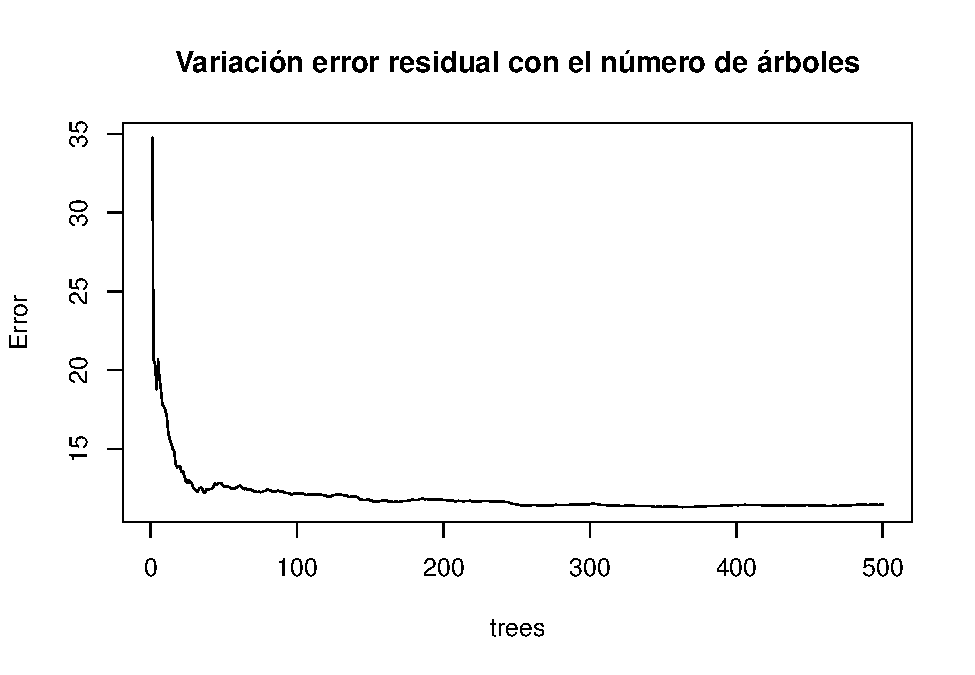
\includegraphics{TrabajoPracticas3_files/figure-latex/unnamed-chunk-51-1.pdf}

Ahora procederemos a calcular el error de test. Para ello usaremos como
en ejercicios anteriores la función predict.

\begin{Shaded}
\begin{Highlighting}[]
\NormalTok{##Realizamos la predicción con 'predict'}
\NormalTok{##introducimos como parámetros el modelo que hemos predicho}
\NormalTok{##con bagging y el subconjunto de test}


\NormalTok{boston.pred <-}\StringTok{ }\KeywordTok{predict}\NormalTok{(boston.model, }\DataTypeTok{newdata =} \NormalTok{dataBoston3[-training,])}

\NormalTok{y.medv <-}\StringTok{ }\NormalTok{dataBoston3$medv[-training]}
\NormalTok{sq.error <-}\StringTok{ }\KeywordTok{mean}\NormalTok{((boston.pred-y.medv)^}\DecValTok{2}\NormalTok{)}

\NormalTok{##El error cuadrático medio es el siguiente}
\NormalTok{sq.error}
\end{Highlighting}
\end{Shaded}

\begin{verbatim}
## [1] 7.77245
\end{verbatim}

\subsection{Apartado c}\label{apartado-c-1}

Ahora para estimar mediante un modelo RandomForest usaemos de nuevo la
misma función que en el apartado anterior. A diferencia del apartado
anterior, ahora usaremos como número de variables para ramificación
\(\frac{p}{3}\) siendo p el número de variables predictoras.

Usamos las mismas particiones para hacer la comparación con bagging en
igualdad de condiciones.

\begin{Shaded}
\begin{Highlighting}[]
\NormalTok{##Apartado c}

\KeywordTok{set.seed}\NormalTok{(}\DecValTok{1}\NormalTok{)}

\NormalTok{boston.rf.model <-}\StringTok{ }\KeywordTok{randomForest}\NormalTok{(}\DataTypeTok{formula=} \NormalTok{dataBoston3$medv ~}\StringTok{ }\NormalTok{., }\DataTypeTok{data=}\NormalTok{dataBoston3, }
                             \DataTypeTok{subset=}\NormalTok{training, }\DataTypeTok{mtry=}\NormalTok{(}\KeywordTok{ncol}\NormalTok{(dataBoston)-}\DecValTok{1}\NormalTok{)/}\DecValTok{3}\NormalTok{, }\DataTypeTok{importance=}\OtherTok{TRUE}\NormalTok{)}

\NormalTok{##Gráfico de la variación del error con el número de árboles}
\KeywordTok{plot}\NormalTok{(boston.rf.model, }\DataTypeTok{main=}\StringTok{"Variación error residual con el número de árboles"}\NormalTok{)}
\end{Highlighting}
\end{Shaded}

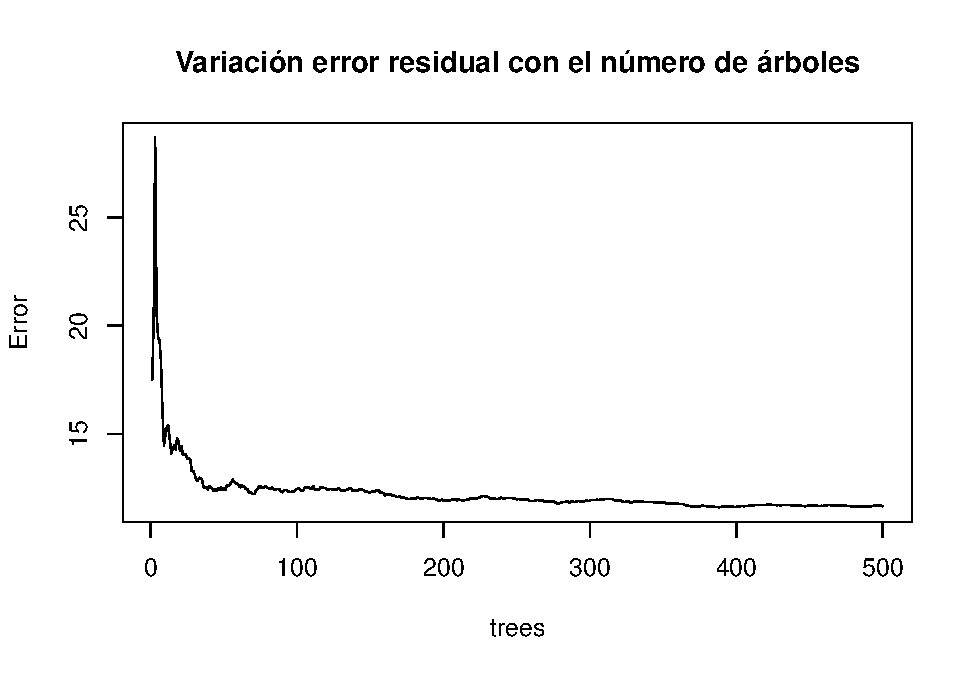
\includegraphics{TrabajoPracticas3_files/figure-latex/unnamed-chunk-55-1.pdf}

He intentado aplicar la funcón tune.randomForest pero no he conseguido
hacerla funcionar.

Ahora calculamos el error de test igual que en el apartado anterior

\begin{Shaded}
\begin{Highlighting}[]
\NormalTok{boston.pred.rf <-}\StringTok{ }\KeywordTok{predict}\NormalTok{(boston.rf.model, }\DataTypeTok{newdata =} \NormalTok{dataBoston3[-training,])}

\NormalTok{y.medv.rf <-}\StringTok{ }\NormalTok{dataBoston3$medv[-training]}
\NormalTok{sq.error.rf <-}\StringTok{ }\KeywordTok{mean}\NormalTok{((boston.pred.rf-y.medv.rf)^}\DecValTok{2}\NormalTok{)}

\NormalTok{##El error de test es el siguiente}
\NormalTok{sq.error.rf}
\end{Highlighting}
\end{Shaded}

\begin{verbatim}
## [1] 8.481
\end{verbatim}

El error en este caso no varía significativamente con respecto al de
`bagging'. En `bagging' el error está sólo un 1\% por debajo que el de
`Random Forest'.

\subsection{Apartado d}\label{apartado-d}

Para aplicar `Boosting' usaremos la función gbm() del paquete gbm. Esta
función ajuta boosting usando árboles de regresión. Usaremos la misma
partición de los datos que en los apartados anteriores para mantenre la
igualdad de condiciones. El argumento distribution =``gaussian'' es para
indicarle que es un problema de regresión. Con n.trees=5000 le indico
que quiero 5000 árboles y cno interaction.depth le digo que el límite de
profundidad por árbol sea 4.

\begin{Shaded}
\begin{Highlighting}[]
\NormalTok{##Apartado d}
\KeywordTok{set.seed}\NormalTok{(}\DecValTok{1}\NormalTok{)}

\NormalTok{boston.boost <-}\StringTok{ }\KeywordTok{gbm}\NormalTok{(}\DataTypeTok{formula=}\NormalTok{dataBoston3$medv[training] ~., }\DataTypeTok{data=}\NormalTok{dataBoston3[training,], }
                    \DataTypeTok{distribution =}\StringTok{"gaussian"}\NormalTok{,}\DataTypeTok{n.trees =}\DecValTok{5000} \NormalTok{, }\DataTypeTok{interaction.depth =}\DecValTok{4}\NormalTok{)}

\KeywordTok{summary}\NormalTok{(boston.boost)}
\end{Highlighting}
\end{Shaded}

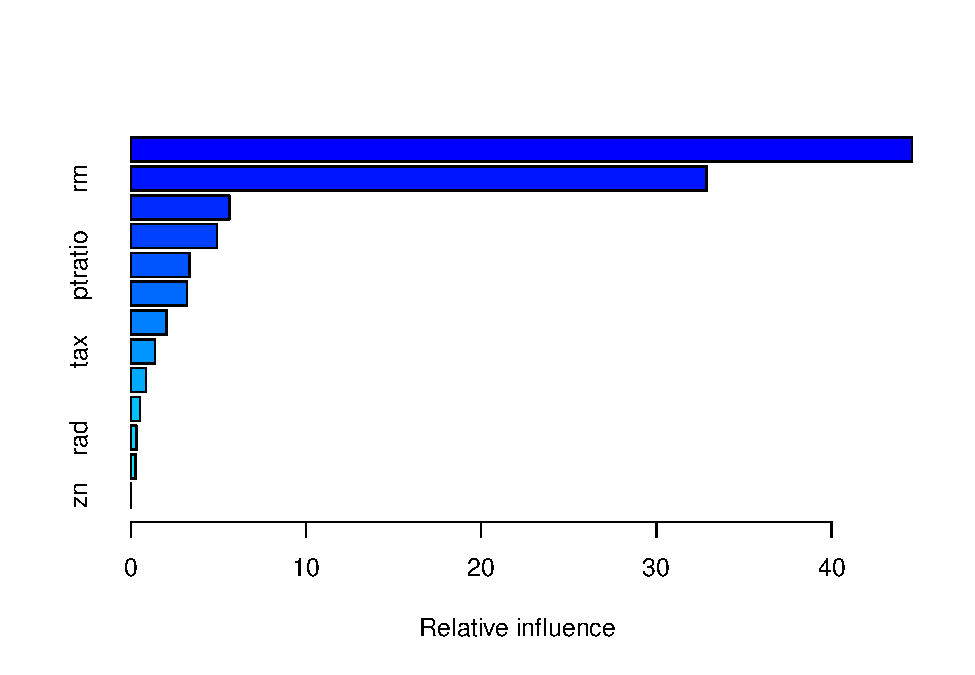
\includegraphics{TrabajoPracticas3_files/figure-latex/unnamed-chunk-59-1.pdf}

\begin{verbatim}
##             var     rel.inf
## lstat     lstat 44.59185317
## rm           rm 32.86765795
## dis         dis  5.62251509
## nox         nox  4.93079948
## ptratio ptratio  3.34634028
## crim       crim  3.20150126
## age         age  2.03491364
## tax         tax  1.37029189
## black     black  0.86988798
## indus     indus  0.53654575
## rad         rad  0.32667686
## chas       chas  0.27783381
## zn           zn  0.02318283
\end{verbatim}

Ahora procedemos a calcular el error de test del modelo. Seguimos los
mismos pasos que en apartados anteriores.

\begin{Shaded}
\begin{Highlighting}[]
\NormalTok{##Hacemos la predicción}

\NormalTok{boston.pred.boost <-}\StringTok{ }\KeywordTok{predict}\NormalTok{(boston.boost, }\DataTypeTok{newdata =} \NormalTok{dataBoston3[-training,], }\DataTypeTok{n.trees=}\DecValTok{5000}\NormalTok{)}
\NormalTok{y.medv.boost <-}\StringTok{ }\NormalTok{dataBoston3$medv[-training]}
\NormalTok{sq.error.boost <-}\StringTok{ }\KeywordTok{mean}\NormalTok{((boston.pred.boost-y.medv.boost)^}\DecValTok{2}\NormalTok{)}

\NormalTok{##El error de test es el siguiente}
\NormalTok{sq.error.boost}
\end{Highlighting}
\end{Shaded}

\begin{verbatim}
## [1] 8.317748
\end{verbatim}

Como vemos, igual que los 2 anteriores modelos, `boosting' presenta para
la misma muestra un error de test similar. Presenta un error
prácticamente igual que en randomForest y sólo un 1\% por encima del de
`bagging'.

\section{Ejercicio 4}\label{ejercicio-4}

Para este ejercicio usaremos la base de datos OJ de la biblioteca ISLR.
Esta base de datos contiene datos sobre zumos de naranja. Lo que tenemos
que hacer primero es crear un conjunto de entrenamiento y posteriormente
elegir la variable `Purchase' como variable que queremos predecir.
Posteriormente ajustaremos un árbol.

\subsection{Apartado a, b y c}\label{apartado-a-b-y-c}

\begin{Shaded}
\begin{Highlighting}[]
\NormalTok{##########EJERCICIO 4}
\CommentTok{#Apartados a, b y c}


\NormalTok{datos4 <-}\StringTok{ }\NormalTok{OJ}

\NormalTok{##Creo un array que serán las variables respuesta}

\KeywordTok{set.seed}\NormalTok{(}\DecValTok{1}\NormalTok{)}

\NormalTok{##creamos la submuestra de 800 observaciones para training}
\NormalTok{training_4 <-}\StringTok{ }\KeywordTok{sample}\NormalTok{(}\DataTypeTok{x=}\DecValTok{1}\NormalTok{:}\KeywordTok{nrow}\NormalTok{(datos4), }\DataTypeTok{size=}\DecValTok{800}\NormalTok{)}

\NormalTok{training.OJ <-}\StringTok{ }\NormalTok{datos4[training_4,]}
\NormalTok{test.OJ <-}\StringTok{ }\NormalTok{datos4[-training_4,]}
\end{Highlighting}
\end{Shaded}

A continuación ajustaremos un árbol a los datos de entrenamiento y lo
dibujamos

\begin{Shaded}
\begin{Highlighting}[]
\CommentTok{#Ajustamos un árbol y lo dibujamos para interpretarlo (interpretación en el pdf)}
\KeywordTok{set.seed}\NormalTok{(}\DecValTok{1}\NormalTok{)}

\NormalTok{tree.OJ <-}\StringTok{ }\KeywordTok{tree}\NormalTok{(training.OJ$Purchase~., training.OJ)}

\KeywordTok{plot}\NormalTok{(tree.OJ)}
\KeywordTok{text}\NormalTok{(tree.OJ, }\DataTypeTok{pretty =} \DecValTok{0}\NormalTok{)}
\end{Highlighting}
\end{Shaded}

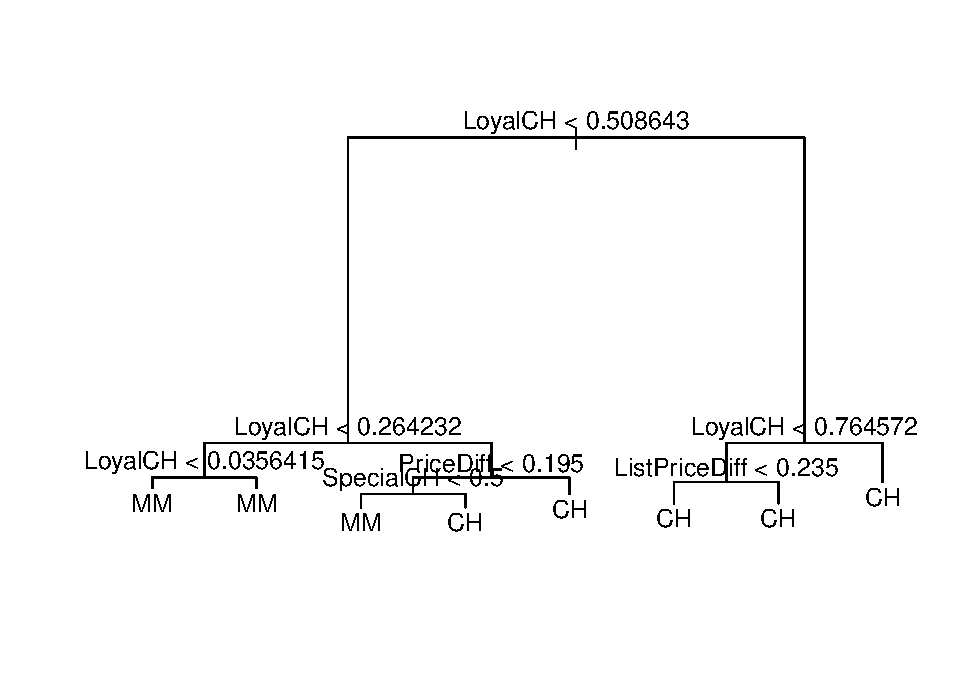
\includegraphics{TrabajoPracticas3_files/figure-latex/unnamed-chunk-64-1.pdf}

El árbol que hemos ajustado usa sólo 4 variables del conjunto de
variables predictoras para ajustarse. Lo que el árbol hace es, si
LoyalCH es mayor que 0.508643, entonces Purchase será CH (con distintas
probabilidades eso sí, dependiendo también posteriormente de
ListPriceDiff). Si es menor de lo que hemos dicho entonces si es menor
que 0.264232 Purchase será MM con distintas probabilidades. Si es mayor,
entonces si PriceDiff es mayor que 0.195 purchase será CH y si es menor,
entonces si SpecialCH es menor de 0.5 será MM y si no será CH.

Ahora analizamos un resumen del ajuste

\begin{Shaded}
\begin{Highlighting}[]
\NormalTok{##Resumen del árbol}

\KeywordTok{summary}\NormalTok{(tree.OJ)}
\end{Highlighting}
\end{Shaded}

\begin{verbatim}
## 
## Classification tree:
## tree(formula = training.OJ$Purchase ~ ., data = training.OJ)
## Variables actually used in tree construction:
## [1] "LoyalCH"       "PriceDiff"     "SpecialCH"     "ListPriceDiff"
## Number of terminal nodes:  8 
## Residual mean deviance:  0.7305 = 578.6 / 792 
## Misclassification error rate: 0.165 = 132 / 800
\end{verbatim}

Como vemos, el árbol usa 4 variables predictoras para ajustar el árbol.
Tiene 8 nodos terminales y 15 nodos en total (contados a partir del
dibujo). El error de training es del 16.5\%.

\subsection{Apartado d}\label{apartado-d-1}

Ahora calcularemos el error de test. Para hacerlo usaremos como en otros
ejercicios anteriores la función predict. Le indico mediante el
parámetro type que se trata de un problema de clasificación.

\begin{Shaded}
\begin{Highlighting}[]
\CommentTok{#Apartado d}

\NormalTok{purchase.pred <-}\StringTok{ }\KeywordTok{predict}\NormalTok{(tree.OJ, }\DataTypeTok{newdata =} \NormalTok{test.OJ, }\DataTypeTok{type=}\StringTok{"class"}\NormalTok{)}

\NormalTok{##Tabla de confusión}
\NormalTok{tabla <-}\StringTok{ }\KeywordTok{table}\NormalTok{(purchase.pred, datos4$Purchase[-training_4])}

\NormalTok{tabla}
\end{Highlighting}
\end{Shaded}

\begin{verbatim}
##              
## purchase.pred  CH  MM
##            CH 147  49
##            MM  12  62
\end{verbatim}

\begin{Shaded}
\begin{Highlighting}[]
\NormalTok{##Calculo la tasa de error de test}

\NormalTok{errores <-}\StringTok{ }\NormalTok{purchase.pred[purchase.pred!=datos4$Purchase[-training_4]]}
\NormalTok{error <-}\StringTok{ }\KeywordTok{length}\NormalTok{(errores)/}\KeywordTok{length}\NormalTok{(purchase.pred)}
\NormalTok{error}
\end{Highlighting}
\end{Shaded}

\begin{verbatim}
## [1] 0.2259259
\end{verbatim}

Como vemos la tasa de error de test es de un 22.59\%. La precisión la
calculamos como:
\(\frac{VerdaderosPositivos}{FalsosPositivos+VerdaderosPositivos}\) en
el caso de la precisión positiva y como
\(\frac{VerdaderosNegativos}{FalsosNegativos + VerdaderosNegativos}\) .
Consideraremos respuestas positivas CH, por lo que la precisión es:
147/(147+49) = 0.75. Hay una precisión positiva del 75\%. La precisión
negativa será 62/(62+12) = 0.8378. La precisión negativa es del 83.78\%.

En cuanto a la tabla de confusión, se puede observar que hay muchos más
falsos negativos que falsos positivos. Esto puede deberse a que en
proporción en el conjunto de training haya más datos `CH' que `MM' y el
árbol se haya ajustado de manera que tienda a coger la clase
mayoritaria.

\subsection{Apartado e}\label{apartado-e}

Ahora mediante la función cv.tree, averiguaremos por validación cruzada
el tamaño óptimo del árbol. A la función le introducimos como parámetro
el árbol anteriormente ajustado con el training set.

\begin{Shaded}
\begin{Highlighting}[]
\CommentTok{#Apartado e}

\CommentTok{#Por validación cruzada comprobamos el mejor árbol}
\NormalTok{tree.cv <-}\StringTok{ }\KeywordTok{cv.tree}\NormalTok{(tree.OJ)}

\KeywordTok{plot}\NormalTok{(tree.cv)}
\end{Highlighting}
\end{Shaded}

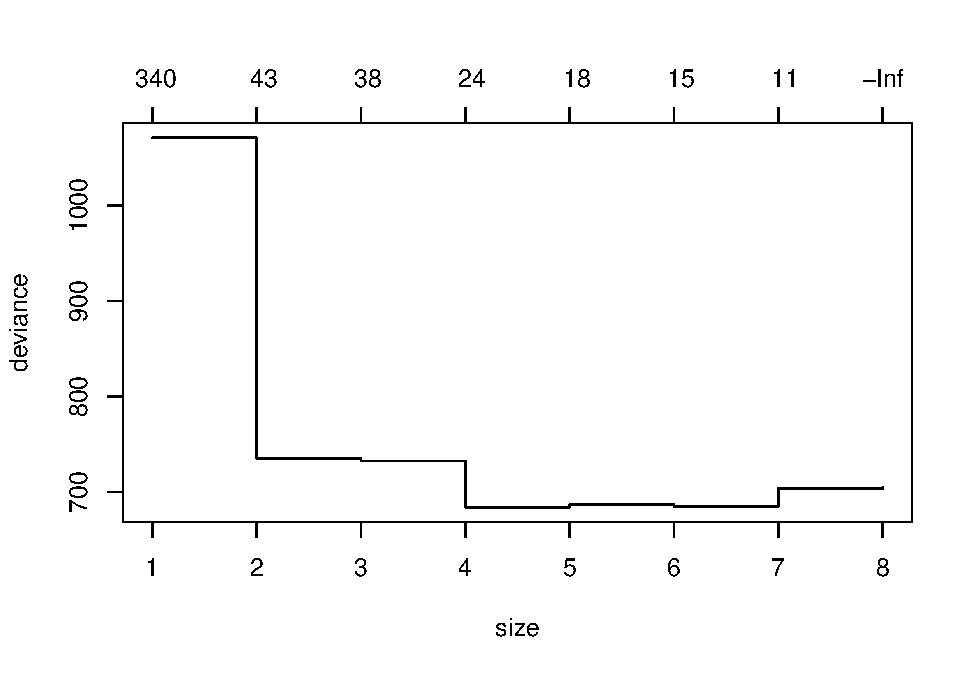
\includegraphics{TrabajoPracticas3_files/figure-latex/unnamed-chunk-72-1.pdf}

Al ver la gráfica, yo cogería el árbol de tamaño que menos desviación
tenga (menos varianza). En este caso según la gráfica es el de tamaño 7,
ya que cuando llega a 8 vuelve a subir la varianza.

\end{document}
